\chapter{Quantum repeaters}
\label{sec:12_quantum_repeaters}
\label{sec:repeaters}

\section{The need for repeaters}
\label{sec:12-1_need_for_repeaters}

In the previous chapter, we saw that there is one big problem when trying to communicate over long distances, and that's photon loss in fibers.
The farther we are trying to communicate, the more likely we are to lose the photon.
There is also another problem: the number of devices that are connected to the network. Currently (2023) there are 8 billion people, and an estimated 31 billion Internet of Things devices.
Despite this staggering number, all of these devices can communicate with each other.
How is this achieved?
One way is to establish a direct connection between each device that is present in the network, as shown in the left panel of Fig.~\ref{fig:12-1_all_to_all}.
Two devices are connected by a single link.
Three devices require three links, four devices require six links and so on.
For $N$ devices, $N (N - 1) / 2$ links are needed in order to have all-to-all coupling.

\begin{figure}[t]
    \centering
    \includegraphics[width=0.85\textwidth]{lesson12/12-1_all_to_all.pdf}
    \caption[All-to-all coupling between network nodes.]{The left panel shows how many links are required to have all-to-all coupling. The right panel shows a more realistic network topology and the path along which a qubit needs to be teleported from sender to a receiver.}
    \label{fig:12-1_all_to_all}
\end{figure}

Real networks do not use all-to-all coupling.
In all-to-all coupling, each individual connection is a link requiring dedicated hardware that enables communication between two devices in the network.
Adding a single device to the network would also require us to add links to every existing device.
Such an approach is clearly not practical even for relatively small networks, let alone worldwide.
The right panel of Fig.~\ref{fig:12-1_all_to_all} shows a much more realistic network, where an arbitrary sender can still transmit a message to the intended receiver, even in the absence of a direct link between the two.

In quantum networks, information encoded in qubits is not transmitted directly.
Rather, we use entangled pairs of qubits to teleport the state of the qubit, as discussed in Chapter~\ref{sec:8_teleportation}.
Each link connecting two devices shares a Bell pair that is used to pass the state of the qubit carrying the quantum message from one device to the next.
We can go back to the right panel of Fig.~\ref{fig:12-1_all_to_all}, and this time think of it as a quantum network, where the quantum sender wishes to pass the state of a qubit to the recipient.
The state of the sender's qubit can be teleported hop-by-hop along the red path until it reaches the recipient.
A problem with this approach is that the operations required by the teleportation protocol as well as the memories used to store Bell pairs are not perfect.
This decreases the fidelity of the teleported qubit.
Repeating the teleportation in this hop-by-hop approach degrades the fidelity of the entangled state, resulting in a garbled quantum state being teleported to the recipient.
One way around this problem is to use the link-level Bell pairs to create a direct entangled connection between the sender and the recipient so that the quantum state can be teleported in one hop.
The quantum nodes tasked with achieving this splicing of link-level entanglement are called \emph{\textbf{quantum repeaters}}\index{quantum repeater}, and they are indispensable in the design of long-distance quantum networks.

We will address four requirements in this chapter.
First, we will show how to establish entanglement between neighboring nodes of a quantum network.
This is known as \textbf{\emph{link-level entanglement}}\index{link-level entanglement}.
Next, we will discuss how the link-level entanglement can be used to create a long-distance entangled connection between end nodes using \textbf{\emph{entanglement swapping}}\index{entanglement swapping}.
After this, we will deal with the issues presented by the adverse effects of noise.
Finally, we will look at management of networks, routing, multiplexing and resource management.


%%%%%%%%%%%%%%%%%%%%%%%%%%%%%%%%%%%%%%%%%%%%%%%%%
\section{Making link-level entanglement}
\label{sec:12-2_making_link_level_rantanglement}
%%%%%%%%%%%%%%%%%%%%%%%%%%%%%%%%%%%%%%%%%%%%%%%%%

In this section, we consider the task of creating link-level entanglement between two neighboring repeaters of a quantum network.
One method for entangling two quantum memories and creating link-level entanglement, known as the \emph{\textbf{memory-interfere-memory}} (MIM)\index{memory-interfere-memory (MIM)} link architecture, is pictured in Fig.~\ref{fig:12-2_MIM}.
Another name for this architecture is ``meet-in-the-middle''.
We tend to avoid using this term to reduce the chance of confusion with man-in-the-middle, which is a type of security attack.
Each repeater node is equipped with a quantum memory, and is coupled to an optical fiber.
The fibers lead to a \emph{\textbf{Bell state analyzer}} (BSA)\index{Bell state analyzer (BSA)}, an optical device which is capable of measuring two incoming photons in the Bell basis.
We will discuss an implementation of the BSA in Section~\ref{sec:13-3_Bell_state_measurement_2}.

\begin{figure}[t]
    \centering
    \includegraphics[width=0.8\textwidth]{lesson12/12-2_MIM.pdf}
    \caption[MIM link architecture.]{Memory-interfere-memory (MIM) link architecture.}
    \label{fig:12-2_MIM}
\end{figure}

The protocol to generate entanglement between the quantum memories is the following.
Each quantum memory emits a photon that is entangled with it, represented by the red dashed line in Step 1 of Fig.~\ref{fig:12-2_MIM}.
These photons are captured and coupled to a fiber, which guides them to the BSA.
At the BSA they are measured in the Bell basis and destroyed in the process.
The success probability of the Bell state measurement depends on the implementation of the BSA.
Straightforward implementation using only linear optics elements results in success probability of at most $50\%$.
This is assuming ideal couplers (to collect photons emitted by the memories), fibers, and detectors at the BSA.
Once the measurement is successful, the entanglement between the memory-photon pairs is transferred to be between the memories as seen in Step 2.

A crucial point about this scheme, and other link-level architectures, is that the photons arriving at the BSA to be measured in the Bell basis must be \textit{\textbf{indistinguishable}}\index{indistinguishable photons}.
This is achieved by arranging for the photons to arrive at the BSA simultaneously, and for the them to have identical spectral properties. 
Even relatively small delays in their arrival times reduce the indistinguishability of the photons, resulting in a diminishing success probability of the Bell state measurement.

\begin{figure}[t]
    \centering
    \includegraphics[width=0.85\textwidth]{lesson12/12-2_MM_MSM.pdf}
    \caption[MM and MSM architectures]{Memory-memory and Memory-source-memory link-level architectures.}
    \label{fig:12-2_MM_MSM}
\end{figure}

Figure~\ref{fig:12-2_MM_MSM} shows two more link-level architectures.
The first one is \textit{\textbf{memory-memory}} (MM)\index{MM link}, where the BSA device is included in one of the repeater nodes.
Entanglement is established in a fashion similar to the MIM architecture, but this time the photon generated by the quantum memory on the left travels the whole length of the fiber to the right node.
There, it interferes with a photon emitted by the right quantum memory.
This architecture sometimes is called ``sender-receiver ''architecture.
The bottom panel of Fig.~\ref{fig:12-2_MM_MSM} shows the \textit{\textbf{memory-source-architecture}} (MSM)\index{MSM link} architecture.
A source of entangled photon pairs is located between the quantum repeaters.
These photons are sent to the quantum repeaters where they interfere with photons emitted locally by the quantum memories. This architecture sometimes is called ``mid-point source'' architecture.


%%%%%%%%%%%%%%%%%%%%%%%%%%%%%%%%%%%%%%%%%%%%%%%%%%%%%%
\section{Reaching for distance: Entanglement swapping}
\label{sec:12-3_reaching_for_distance}
%%%%%%%%%%%%%%%%%%%%%%%%%%%%%%%%%%%%%%%%%%%%%%%%%%%%%%

In the previous section, we saw how to establish link-level entanglement.
We will now extend it to establishing long-distance entanglement spanning multiple hops.
Consider three network nodes represented by Repeater 0, Repeater 1, and Repeater 2, as pictured in Fig.~\ref{fig:12-3_entanglement_swapping}.
Repeaters 0 and 2 each have one qubit, while Repeater 1 has two.
We assume that link-level entanglement has been established between Repeater 0 and one of the qubits at Repeater 1, and the other qubit at Repeater 1 and Repeater 2.
The goal is to establish entanglement between Repeater 0 and Repeater 2.

\begin{figure}[t]
    \centering
    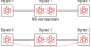
\includegraphics[width=0.8\textwidth]{lesson12/12-3_entanglement_swapping.pdf}
    \caption[Entanglement swapping.]{Entanglement swapping at Repeater 1 creates entanglement between Repeaters 0 and 2.}
    \label{fig:12-3_entanglement_swapping}
\end{figure}

This is achieved by measuring the two qubits at Repeater 1 in the Bell basis.
This measurement projects them onto one of the four Bell pairs.
At the same, the effect of this measurement is to also project the qubits at Repeater 0 and Repeater 2 onto a Bell pair, creating entanglement between these two distant repeaters.
This procedure is known as \emph{\textbf{entanglement swapping}}\index{entanglement swapping}, and it is an indispensable tool in creating long-distance entanglement in quantum networks.
This entanglement is between two repeaters which are not directly connected.

Let's now get a little technical and show more rigorously that Repeater 0 and Repeater 2 are indeed entangled.
We label the qubit at Repeater 0 $A$, and the qubit with which it is entangled at Repeater 1 $A^{\prime}$.
The other qubit at Repeater 1 is denoted by $B^{\prime}$, and its entangled partner at Repeater 2 by $B$.
The state of the $AA^{\prime}$ qubits is one of the Bell pairs, let's say $|\Phi^+\rangle$.
The same goes for the pair of qubits $BB^{\prime}$.
The total state of the four qubits can therefore be written as
\begin{align}
    \begin{aligned}
        \ket{\psi}_{AA^{\prime}B^{\prime}B} & = \ket{\Phi^{+}}_{A A^{\prime}}\ket{\Phi^{+}}_{B^{\prime} B} \\
        & = \frac{1}{2} ( |0000\rangle+|0011\rangle+|1100\rangle+|1111\rangle ).
        \label{eq:12-3_computational_basis}
    \end{aligned}
\end{align}

In the next step of our calculation, we will use a little trick.
We rewrite the state of the qubits at Repeater 1, $A^{\prime}B^{\prime}$, as superpositions of the Bell states,
\begin{align}
    |00\rangle & = \left( |\Phi^{+}\rangle + |\Phi^{-}\rangle\right) / \sqrt{2}, \\
    |01\rangle & = \left( |\Psi^{+}\rangle + |\Psi^{-}\rangle\right) / \sqrt{2}, \\
    |10\rangle & = \left( |\Psi^{+}\rangle - |\Psi^{-}\rangle\right) / \sqrt{2}, \\
    |11\rangle & = \left(|\Phi^{+}\rangle - |\Phi^{-}\rangle\right) / \sqrt{2}.
\end{align}
We can now substitute these identities in Eq.~\ref{eq:12-3_computational_basis}, and rewrite the total state of the four qubits as follows,
\begin{align}
    |\psi\rangle_{AA^{\prime}B^{\prime}B} = & \frac{1}{2} \Biggl[ |0\rangle \underbrace{\frac{|\Phi^+\rangle + |\Phi^-\rangle}{\sqrt{2}}}_{=\ket{00}} |0\rangle + |0\rangle \underbrace{\frac{|\Psi^+\rangle + |\Psi^-\rangle}{\sqrt{2}}}_{=\ket{01}} |1\rangle \nonumber\\
    & + |1\rangle \underbrace{\frac{|\Psi^+\rangle - |\Psi^-\rangle}{\sqrt{2}}}_{=\ket{10}} |0\rangle + |1\rangle \underbrace{\frac{|\Phi^+\rangle - |\Phi^-\rangle}{\sqrt{2}}}_{=\ket{11}} |1\rangle \Biggr].
\end{align}
We can group the qubits that are going to be measured on the left, and the qubits that we are not going to measure on the right,
\begin{align}
    |\psi\rangle_{A^{\prime}B^{\prime}AB} = & \frac{1}{2} \left[ \frac{|\Phi^+\rangle + |\Phi^-\rangle}{\sqrt{2}}|0\rangle|0\rangle + \frac{|\Psi^+\rangle + |\Psi^-\rangle}{\sqrt{2}}|0\rangle|1\rangle \right. \nonumber\\
    & + \left. \frac{|\Psi^+\rangle - |\Psi^-\rangle}{\sqrt{2}}|1\rangle|0\rangle + \frac{|\Phi^+\rangle - |\Phi^-\rangle}{\sqrt{2}}|1\rangle|1\rangle \right].
\end{align}
We have not really done anything apart from rearranging the qubits.
Finally, we collect all terms with the same Bell pair on qubits $A^{\prime}B^{\prime}$,
\begin{align}
    |\psi\rangle_{A^{\prime}B^{\prime}AB} = & \frac{1}{2} \left[ |\Phi^+\rangle \frac{|0\rangle|0\rangle + |1\rangle|1\rangle}{\sqrt{2}} + |\Psi^+\rangle \frac{|0\rangle|1\rangle + |1\rangle|0\rangle}{\sqrt{2}} \right. \nonumber\\
    & + \left. |\Psi^-\rangle \frac{|0\rangle|1\rangle - |1\rangle|0\rangle}{\sqrt{2}} + |\Phi^-\rangle \frac{|0\rangle|0\rangle - |1\rangle|1\rangle}{\sqrt{2}} \right].
    \label{eq:12-3_almost_final}
\end{align}
Looking at the state of qubits $AB$ in Eq.~(\ref{eq:12-3_almost_final}), we recognize that the qubits are in fact entangled.
We can make this even more explicit,
\begin{align}
    |\psi\rangle_{A^{\prime}B^{\prime}AB} & = \frac{1}{2} \left[ |\Phi^+\rangle |\Phi^+\rangle + |\Psi^+\rangle |\Psi^+\rangle + |\Psi^-\rangle |\Psi^-\rangle + |\Phi^-\rangle |\Phi^-\rangle \right].
    \label{eq:12-3_final}
\end{align}

We can see that if the Bell-state measurement at Repeater 1 results in the outcome $|\Phi^+\rangle_{A^{\prime}B^{\prime}}$, then the state of the qubits at Repeaters 0 and 2 is $|\Phi^+\rangle_{AB}$.
Similarly if the measurement outcome at Repeater 1 is $|\Psi^+\rangle_{A^{\prime}B^{\prime}}$, then Repeaters 0 and 2 share the state $|\Psi^+\rangle_{AB}$, and so on for the other measurement outcomes.

We see that the outcome of the Bell-state measurement is not deterministic.
Each possibility can occur with equal probability of $1/4$.
Performing only the measurement is not enough to distribute entanglement between Repeaters 0 and 2.
Remember, that the measurement takes place far away from Repeaters 0 and 2.
The outcome of the measurement must be communicated to them via a \emph{\textbf{classical message}}.
Only after receiving this message from Repeater 1 will they share a pure Bell pair.
Repeater 1 does not need to send the outcome of the measurement to both Repeaters 0 and 2.
It is enough to send it just to one of them, but both of the Repeaters need to be notified that the procedure has been carried out successfully.
This introduces a time delay that limits how fast the process of establishing entanglement can progress.

Maybe you have noticed that entanglement swapping is very similar to creation of link-level entanglement described in Section~\ref{sec:12-2_making_link_level_rantanglement}.
Mathematically the two procedures are very similar.
At the  link level, memory-photon entanglement is swapped by measuring the photons at the Bell state analyzer, creating memory-memory entanglement.
Whereas in end-to-end entanglement, we are only swapping entanglement between between pairs of memories.
Physically, this is quite a big difference: using linear optics, the maximum success probability of performing entanglement swapping on photons is limited to $50\%$, but entanglement swapping between memories can be done \textbf{\emph{deterministically}}, provided that we have good experimental techniques and we can limit the effects of noise.

An alternative way of understanding entanglement swapping is through teleportation.
By measuring its two qubits in the Bell basis, Repeater 1 is really teleporting the state of qubit $A^{\prime}$ to qubit $B$.
Since qubit $A^{\prime}$ is entangled with the qubit at Repeater 0, this entanglement is also transferred to Repeater 2 along with the state of qubit $A^{\prime}$.



%%%%%%%%%%%%%%%%%%%%%%%%%%%%%%%%%%%%%%%%
\section{Detecting errors: purification}
\label{sec:12-4_purification}
%%%%%%%%%%%%%%%%%%%%%%%%%%%%%%%%%%%%%%%%

In this section, we will address what happens when we also include errors in our considerations.
We will learn how to  handle these errors and create a state between Repeater 0 and Repeater 2 of acceptable fidelity.
Our desired state that we want to share between Repeater 0 and 2 is given by the maximally entangled state $\ket{\Phi^+}$.
In the density matrix form, we write it as the outer product,
\begin{align}
    \rho_{AB} = \ket{\Phi^{+}}\bra{\Phi^{+}}.
\end{align}
In reality, there will always be some noise affecting the system.
The state $\rho_{AB}$ will be a mixture of the desired pure state $\ket{\Phi^+}$, and some other unwanted noisy term $\rho_{\text{noise}}$.
With probability given by the fidelity $F$, we will have the desired state $\ket{\Phi^+}$, and with probability $1-F$, we will have some noisy state $\rho_{\text{noise}}$,
\begin{align}
    \rho_{AB} = F |\Phi^{+}\rangle\langle\Phi^{+}|+(1-F)\rho_{\text{noise}}.
\end{align}

Rather than considering the general case of how noise affects our maximally entangled state, we will consider the specific example of a bit-flip channel, which we saw in Sec.~\ref{sec:3-3_density_matrices}.
This channel leaves the state unaffected with probability $F$, otherwise it applies the Pauli $X$ operator to one of the qubits,
\begin{align}
    \rho_{AB} & = F|\Phi^{+}\rangle\langle\Phi^{+}|+(1-F) X_A| \Phi^{+}\rangle\langle\Phi^{+}| X_A \nonumber\\
    & = F \left|\Phi^{+}\right\rangle\left\langle\Phi^{+}|+(1-F)| \Psi^{+}\right\rangle\left\langle\Psi^{+}\right|.
    \label{eq:12-4_bitflip_mixed_state}
\end{align}
We have applied the bit-flip channel to qubit $A$, but it does not matter whether we apply it to qubit $A$ or $B$.
We can easily check that applying the Pauli $X$ operator on qubit $B$ yields the same expression for the state $\rho_{AB}$.

Keep in mind that this is just one possible source of error out of many.
One way of dealing with errors is to use \textbf{\emph{quantum error correction}}\index{quantum error correction (QEC)}.
QEC can detect and correct errors, but usually comes with a large overhead.
Here, we will look at a less ambitious procedure of simply detecting errors, known as \textit{\textbf{purification}}\index{purification}.

Purification is a test for the state $\rho_{AB}$ that checks whether the state is affected by an error.
The test is not perfect and sometimes succeeds even when the state has undergone an error.
If the probability of this ``false positive'' is low enough, then the overall fidelity of the state increases.
It is this sense that we say that the state has been purified.

There are two important things that we need to keep in mind when designing the purification procedure.
First, measurements can be used to reveal information about the state, but they are also very intrusive and destroy the entanglement that we are trying to preserve.
Second, the two qubits of the entangled state are spatially separated and held in separated repeaters.
This distance can be of the order of tens of kilometers for a link, or much longer over a network.

We can get around the first issue of destructive measurement by using another Bell pair to test whether the original pair has undergone the unwanted Pauli $X$ flip.
This is done by entangling the second pair with the original one, and then measuring the second pair in order to extract useful information about the first pair without destroying it.
The second issue of the qubits being at distant locations can be overcome by simple classical communication.

\begin{figure}[t]
    \centering
    \includegraphics[width=0.7\textwidth]{lesson12/12-4_purification.pdf}
    \caption[Entanglement purification for Pauli X errors.]{Entanglement purification for detecting Pauli $X$ errors. In this diagram, each line represents a Bell pair, rather than a single qubit, shared between Alice ande Bob.}
    \label{fig:12-4_purification}
\end{figure}
Let's introduce the detailed protocol for entanglement purification for the Pauli $X$ error, pictured in Fig.~\ref{fig:12-4_purification}.
The horizontal wires represent Bell pairs shared between Alice and Bob.
Ideally, these states are $\ket{\Phi^+}_1$ and  $\ket{\Phi^+}_2$, but due to noise they will be mixed states $\rho_1$ and $\rho_2$.
Alice applies a CNOT gate on the qubits in her possession.
Her qubit from the first pair acts as the control and her qubit from the second pair is the target.
Bob also performs a CNOT gate on his two qubits with the same control/target choice.
Alice and Bob then measure the qubits of the second pair in the Pauli $Z$ basis and send the measurement outcomes to each other using classical messages.
They keep the first pair if the measurement outcomes are the same, meaning they both measured the state \ket{0} or they both measured the state \ket{1}.
We say that the measurement outcomes are \textbf{\emph{correlated}}.
Otherwise they discard the first pair, as different measurement outcomes signal that an error has been detected.

Why this particular sequence of steps works will become more clear when we write them out step-by-step.
We start by considering the ideal case where Alice and Bob share two copies of \ket{\Phi^+}.
We label the two qubits that are sent to Alice as $A_1$ and $A_2$, while Bob's qubits are $B_1$ and $B_2$.
Expanding the initial state and applying the CNOT gates,
\begin{align}
    |\Phi^{+}\rangle_{1} |\Phi^{+}\rangle_{2} & = (|00\rangle + |11\rangle)_{A_1B_1} (|00\rangle + |11\rangle)_{A_2B_2} \nonumber\\
    & = |00\rangle_{A_1B_1} |00\rangle + |00\rangle |11\rangle + |11\rangle |00\rangle +|11\rangle |11\rangle \nonumber\\
    & \stackrel{\mathrm{CNOT}_{A}}{\longrightarrow} |00\rangle|00\rangle+|00\rangle|11\rangle+|11\rangle|10\rangle+|11\rangle|01\rangle \\
    & \stackrel{\mathrm{CNOT}_{B}}{\longrightarrow} |00\rangle|00\rangle+|00\rangle|11\rangle+|11\rangle|00\rangle+|11\rangle|11\rangle \nonumber \\
    & = |\Phi^{+}\rangle_{1} |\Phi^{+}\rangle_{2} \nonumber.
    \label{eq:12-4_purification_ideal}
\end{align}
In the above, we have omitted the normalization constants for clarity.
We see that the CNOT gates have left our initial state unaffected.
Measuring the second pair in the Pauli $Z$ basis will give us the state \ket{00} with probability $1/2$, or the state \ket{11} with probability of $1/2$.
The outcomes will always be correlated and therefore Alice and Bob will always keep the first pair.
As well as they should since the first pair is not affected by an error.

Let's see what happens when the first pair is affected by a Pauli $X$ error.
Repeating the same calculation as in Eq.~(\ref{eq:12-4_purification_ideal}), we get
\begin{align}
    |\Psi^{+}\rangle_{1} |\Phi^{+}\rangle_{2} & = (|01\rangle + |10\rangle)_{A_1B_1} (|00\rangle + |11\rangle)_{A_2B_2} \nonumber\\
    & = |01\rangle |00\rangle + |01\rangle |11\rangle + |10\rangle |00\rangle +|10\rangle |11\rangle \nonumber\\
    & \stackrel{\mathrm{CNOT}_{A}}{\longrightarrow} |01\rangle|00\rangle+|01\rangle|11\rangle + |10\rangle|10\rangle+|10\rangle|01\rangle \\
    & \stackrel{\mathrm{CNOT}_{B}}{\longrightarrow} |01\rangle|01\rangle+|01\rangle|10\rangle+|10\rangle|10\rangle+|10\rangle|01\rangle \nonumber \\
    & = |\Psi^{+}\rangle_{1} |\Psi^{+}\rangle_{2} \nonumber.
    \label{eq:12-4_purification_error}
\end{align}
This time the error from the first pair has propagated onto the second pair.
Measuring the second pair now yields either \ket{01} or \ket{10}, both with equal probability of $1/2$.
Since the measurement outcomes are anti-correlated, Alice and Bob discard the first pair.

Now we are in a position where we can consider both initially distributed pairs to be in the mixed state given by Eq.~(\ref{eq:12-4_bitflip_mixed_state}),
\begin{equation}
    \rho_1 \otimes \rho_2 = \left[ F |\Phi^+\rangle \langle\Phi^+| + (1 - F) |\Psi^+\rangle \langle\Psi^+| \right]_1 \otimes \left[ F |\Phi^+\rangle \langle\Phi^+| + (1 - F) |\Psi^+\rangle \langle\Psi^+| \right]_2.
\end{equation}
We have already covered the situation where both Bell pairs are unaffected by noise, which occurs with probability of $F^2$, and where the first pair is bit-flipped, occurring with probability of $(1-F)F$.
The remaining two possibilities of only the second pair being bit-flipped and both pairs being bit-flipped can be calculated in exactly same way.
We summarize all 4 possibilities in Tab.~\ref{tab:12-4_purification_X_error}.
\begin{table}[t]
    \setcellgapes{3pt}
    \renewcommand\theadfont{}
    \makegapedcells
    \centering
    \begin{tabular}{cccccc}
        \hline
        \textbf{Pair 1} & \textbf{Pair 2} & \textbf{Probability} & \textbf{Measurement result} & \textbf{Action} & \textbf{Result} \\
        \hline
        $\left|\Phi^{+}\right\rangle$ & $\left|\Phi^{+}\right\rangle$ & $F^{2}$ & 00 or 11 & \textcolor{mygreen}{Keep} & $\left|\Phi^{+}\right\rangle$ \\
        $\left|\Phi^{+}\right\rangle$ & $\left|\Psi^{+}\right\rangle$ & $F(1-F)$ & 01 or 10 & \textcolor{myred}{Discard} & N/A \\
        $\left|\Psi^{+}\right\rangle$ & $\left|\Phi^{+}\right\rangle$ & $(1-F) F$ & 01 or 10 & \textcolor{myred}{Discard} & N/A \\
        $\left|\Psi^{+}\right\rangle$ & $\left|\Psi^{+}\right\rangle$ & $(1-F)^{2}$ & 00 or 11 & \textcolor{mygreen}{Keep} & $\left|\Psi^{+}\right\rangle$ \\
        \hline
    \end{tabular}
    \caption[X error purification]{Purification for a Pauli $X$ error.}
    \label{tab:12-4_purification_X_error}
\end{table}

We can make an interesting observation.
When both initial pairs are affected by Pauli $X$ errors, the purification procedure still tells Alice and Bob to keep the first pair because the measurement outcomes on the second pair are correlated.
This occurs with probability $(1-F)^2$ and is the ``false positive'' that we mentioned earlier in this section.

We can see from Tab.~\ref{tab:12-4_purification_X_error} that the total success probability of this purification procedure is
\begin{equation}
    \text{Pr} \{\text{success}\} = F^2 + (1 - F)^2.
\end{equation}
The state that Alice and Bob share after a successful purification is
\begin{equation}
    \rho' = F' |\Phi^+\rangle\langle\Phi^+| + (1 - F') |\Psi^+\rangle\langle\Psi^+|,
\end{equation}
where the new fidelity $F'$ is related to the initial one via
\begin{align}
    F^{\prime}=\frac{F^{2}}{F^{2}+(1-F)^{2}}.
\end{align}
The expression for the new post-purification fidelity is very interesting.
When $F > 0.5$, the fidelity of the purified state increases, $F' > F$.
The name for the process, purification, is now more clear.
We start with a noisy state and end up with a new state of higher fidelity, a more pure state.



%%%%%%%%%%%%%%%%%%%%%%%%%%%%%
\section{Making a network}
\label{sec:making-a-network}
%%%%%%%%%%%%%%%%%%%%%%%%%%%%%

We have considered two important ingredients that are needed to make a network.
We looked at how to create link-level entanglement between neighboring nodes, and how to extend it to end-to-end entanglement with entanglement swapping.
There are a few missing parts however.
The main two are routing routing, and multiplexing.

At the beginning of this chapter, we saw in Fig.~\ref{fig:12-1_all_to_all} that the job of a quantum network is to establish end-to-end entanglement between distant nodes, which is then consumed by applications.
The network needs a way of picking a suitable path along which to execute entanglement swapping that leads to this end-to-end connection.
The second issue is that the figure shows only one connection request being considered.
Of course, a network will most likely be used by more than one application at a time.
Therefore, the network should be able to satisfy multiple simultaneous connection requests between distinct end nodes.

\begin{figure}[t]
    \centering
    \includegraphics[width=0.8\textwidth]{lesson12/12-5_routing_multiplexing.pdf}
    \caption[Routing and multiplexing.]{Picking the best path along which to entanglement swap is the job of routing. The quantum network also needs to decide how to allocate its scarce resources in order to satisfy multiple simultaneous connection requests.}
    \label{fig:12-5_routing_multiplexing}
\end{figure}

How the network picks an appropriate path where it performs entanglement swapping is determined by the \emph{\textbf{routing algorithm}}\index{routing algorithm} using information about the topology and condition of the network.
The left panel of Fig.~\ref{fig:12-5_routing_multiplexing} shows a simple case of a quantum network with five nodes.
Let's say that nodes A and E would like to establish an entangled connection.
There are three possible paths that the network can choose.
It can swap entanglement at node B (option 1), or at node D (option 2), or at nodes C and D (option 3).
Each option requires the establishment of different patterns of link-level entanglement.
Option 1 requires link-level entanglement between A-B and B-E before the entanglement swapping can be executed.
Similarly, option 3 requires link-level entanglement on the A-D, D-C, and C-E links.

In order to evaluate which path is best, we need to look at the cost for establishing the corresponding link-level entanglement, and then how to combine these costs in order to establish the cost for the entire path.
One possible way to evaluate the link-level entanglement is \emph{\textbf{seconds per Bell pair at a threshold fidelity}}.
We discussed how establishing a link-level entanglement involves photon emission from quantum memories, and subsequent measurement of these photons in the Bell basis.
These processes are all probabilistic, and so is loss of the photons in fiber.
Depending on the properties of the fiber as well as the quantum hardware at each node, the average time required to successfully establish link-level Bell pair will vary.

How do we combine these costs for each individual link in order to know the full cost of establishing end-to-end entanglement over a path?
One possibility is to use \emph{\textbf{Dijkstra's shortest path first algorithm}}\index{Dijkstra's shortest path first}\label{dijkstra}.
We can sum the link-level costs for an individual path in order to estimate the total cost.
We have seen that sometimes we need to purify Bell pairs, which reduces our effective throughput by at least a factor of two.
In order to balance the trade off between the rate of making raw Bell pairs and fidelity and make the comparison between two links fair, we demand that the link-level Bell pairs be of certain threshold fidelity, achieved using purification if necessary.
The exact value of this threshold is dictated by the needs of the application that is requesting the Bell pairs.

The next issue that networks have to deal with is \emph{\textbf{multiplexing}}\index{multiplexing}.
The network will have to satisfy multiple simultaneous connection requests for end-to-end entanglement.
A good multiplexing scheme helps the network decide how to allocate its resources to satisfy these requests in a timely, reliable and fair manner.
The right panel of Fig.~\ref{fig:12-5_routing_multiplexing} shows four simultaneous requests for entanglement between nodes A-K, B-J, C-H, and D-G.
All of these requests need to use link-level entanglement between E-F, creating \textbf{\emph{contention}}\index{contention} on this link.
Another link with contention is F-I, although only two connections need to use that link.
The network must know how to handle such requests, where a single link needs to be shared between multiple users or connections.

In this chapter, we have seen the four requirements for building a quantum network.
We started with the basic building block of establishing link-level entanglement between neighboring nodes of a network and how to handle photon losses.
Next, we discussed how to use entanglement swapping to splice the link-level entanglement into long-distance end-to-end connections between non-neighboring nodes.
Finally, we briefly discussed routing and multiplexing in quantum networks.





\newpage
\begin{exercises}
\exer{
\emph{Fully connected networks.}
How many connections are needed for a fully connected network covering all of the IoT devices in the global classical Internet?
}

\exer{
\emph{Entanglement swapping with projectors.}
We demonstrated that the procedure for entanglement swapping between qubits $AB_1$ and $B_2C$ works by rewriting the state of qubit $B_1$ and $B_2$ in the bell basis.
Let's go through the derivation again but using the formalism of projectors. (If you need to get a refresher on projectors, take a look at the Exercises in Chapter \ref{sec:3_pure_mixed}.)
\subexer{
The initial state of the two entangled pairs is
\begin{equation}
    \ket{\psi} = \ket{\Phi^+}_{AB_1} \ket{\Phi^+}_{B_2C}.
\end{equation}
Write down the set of four projectors corresponding to the four possible measurement outcomes at Node $B$.
}
\subexer{
Compute the probabilities of the four measurement outcomes using the these projectors.
}
\subexer{
Write down the post-measurement states of qubits $AC$ corresponding to the four measurement outcomes using the projectors.
}
}

\exer{
\emph{Entanglement swapping with noisy states.}
Consider the case where the link-level entangled state between Nodes $A$ and $B$ is not the pure Bell pair \ket{\Phi^+}, but is affected by the bit flip channel.
The Bell pair shared between Nodes $B$ and $C$ remains noiseless.
\subexer{
If the fidelity of the Bell pair between Nodes is $A$ and $B$ if $F_{AB}$, write down the total initial state.
}
\subexer{
Write down the probabilities of the four outcomes of the measurements performed by Node $B$.
}
\subexer{
What are the corresponding post-measurement states of qubits $A$ and $C$?
}
\subexer{
How do the fidelities of the post-measurement states of qubits $A$ and $B$ depend on the fidelity $F_{AB_1}$ of the initial link-level entanglement? 
}
\subexer{
Consider the case where the both entangled links are affected by the bit flip channel, and have fidelities $F_{AB_1}$ and $F_{B_2C}$.
Compute the fidelity of the pair $AC$ obtained after entanglement swapping as a function of these initial fidelities.
}
}

\exer{
\emph{Entanglement swapping and MIM link architecture.}
Recall that in the MIM link architecture, quantum memories are made to emit photons, which are then measured at the BSA, creating entanglement between the quantum memories.
This architecture relies on entanglement swapping performed on photonic and matter qubits.
Fig.~(TODO) shows a simplified atomic structure of the a quantum memory emitting a photon.
If the memory transitions from the excited state \ket{e} to the ground state \ket{a_1}, it emits a horizontally polarized photon \ket{H}\footnote{To be precise, the memory emits a circularly polarized photon which is then converted to a linearly polarized photon.}.
If the memory transitions to ground state \ket{a_2}, it emits a vertically polarized photon \ket{V}.
\subexer{
Write down the state of the memory-photon pair, given that the memory is equally likely to transition to states \ket{a_1} and \ket{a_2}.
}
\subexer{
Write down the total state of both memory-photon pairs.
Keep good track of the physical systems with subscripts.
}
\subexer{
The two photons travel to the BSA where they get measured in the Bell basis.
Write down the projectors corresponding to this measurement.
}
\subexer{
What are the post-measurement states of the quantum memories?
}
\noindent The situation is actually more complicated than this.
Bell-state measurement on photonic qubits cannot be implemented deterministically.
Linear optics elements cannot distinguish all four photonic Bell pairs.
We will learn why this is the case in our next book.
}

\exer{
\emph{Purification and Pauli $Z$ errors.}
We described the purification procedure on Bell pairs affected by the bit flip channel.
Let's look at what happens when the Bell pairs undergo a Pauli $Z$ error.
\subexer{
Assume that only Alice's qubit $A_1$ is affected by the Pauli $Z$.
Write down the total state of both Bell pairs.
}
\subexer{
Apply the purification procedure.
Is this the result you expected?
}
\subexer{
If both Bell pairs are mixed states of fidelity $F$, what is the fidelity of the Bell pair after successful purification procedure?
}
}


\end{exercises}

